\section{Parallel loop dependencies with OpenMP \punkte{15}}

In the first parallel version (Listing~\ref{lst:recur_chunk}), we break the index range into separate chunks. Each thread starts off by calculating the initial value with a single \texttt{pow(up, start)} call and then moves on to do local multiplications. This approach uses \texttt{firstprivate(Sn)} to make sure that each thread is working with different indices. \\

The second version (Listing~\ref{lst:recur_dyn}) checks for gaps in the assigned blocks by looking at consecutive indices. Threads \textbf{only} recalculate \texttt{Sn} with \texttt{pow(up, i)} when it's really needed.

\lstinputlisting[
    language=C,
    numbers=left,
    caption={Parallel recurrence with chunk partitioning},
    captionpos=b,
    label={lst:recur_chunk},
    linerange={21-36},
    firstnumber=21
]{../Skeleton\_codes/loop-dependencies/recur_omp.c}

\lstinputlisting[
    language=C,
    numbers=left,
    caption={Parallel recurrence with on-demand recomputation},
    captionpos=b,
    label={lst:recur_dyn},
    linerange={39-52},
    firstnumber=39
]{../Skeleton\_codes/loop-dependencies/recur_omp.c}

The scaling study (Figure~\ref{fig:recur_scaling}) shows that the chunk-based version achieves nearly linear speedup up to 16 threads but then starts to plateau. In contrast, the version with the discontinuity check is slower due to overhead of constant check but it appears to maintaint linearity from 16 to 20 threads on the contrary of the first one. It would be really interesing to try how it goes on on  a machine with more cores.

\begin{figure}[H]
    \centering
    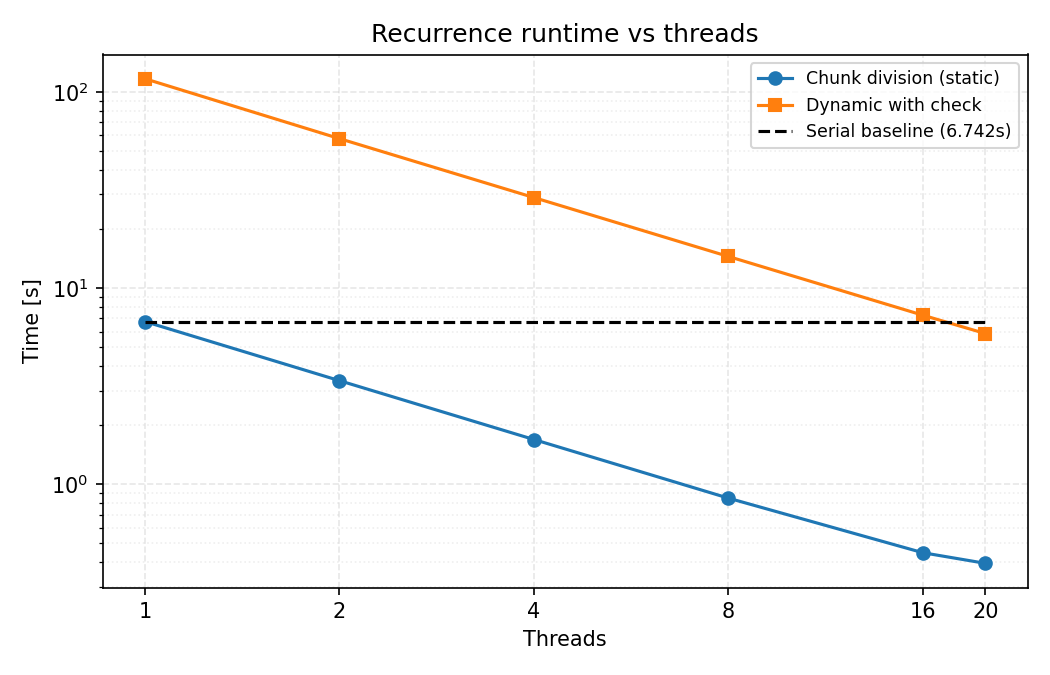
\includegraphics[width=0.75\linewidth]{../Skeleton\_codes/loop-dependencies/plots/recur_runtime_scaling.png}
    \caption{Runtime per thread count for the chunk and dynamic variants, compared with the serial baseline.}
    \label{fig:recur_scaling}
\end{figure}
